\chapter{Introduction}

\section{Motivation}

\paragraph{} There exist many programs for music notation and composition. Sibelius allows users to write scores using traditional western music notation, whilst music is produced in the live programming interface Sonic Pi by real-time editing of Ruby code \cite{aaron:pi}. These require users to gain familiarity with a new interface, often with a large threshold to creating simple musical ideas. Spreadsheet users significantly outnumber programmers \cite{scaffidi:estimating} being the preferred programming language for many people \cite{blackwell:functions}. I believe that this ubiquitousness, along with the affordances of the spreadsheet, would enable new ways to interact with musical notation that capitalise on existing familiarities with spreadsheets and their data handling capabilities.

\paragraph{} The use of grid structures is an established concept in music programs, with most sequencing software using one axis of the screen for time and the other for pitch or musical parts. Chris Nash's Manhattan \cite{nash:manhattan} uses a grid structure where formulae can be defined in the cells to change the cell value, much like in a spreadsheet. However it is limited to columns defining tracks and rows corresponding to different times. Advait Sarkar's SheetMusic \cite{sarkar:sheetmusic} investigated how formulae with sound output can be included within the spreadsheet paradigm. This also introduced abstracting time away from the grid, in this case using an incrementing global \texttt{tick} variable which could be referred to in the formulae. Both axes can be used interchangeably for SheetMusic notation or markup that the user wishes to include which is not interpreted musically, a concept idiomatic to Excel usage. Simple formulae such as \texttt{if(tick\%2==0) p('snare') else p('kick')} allow musical structures to be defined without advanced programming knowledge but quickly become unwieldy for defining larger pieces, especially if they are not highly repetitive. Whilst other spreadsheet music projects exist \cite{hackaday:spreadsheet}, these simply use the spreadsheet as the medium for conventional sequencing with an auxiliary script used to parse the grid and create musical output.

\paragraph{} Excello is an Excel add-in for end-user music programming where users define music in the spreadsheet and can play it back from within Excel. It maintains the abstraction of time from the grid to keep the flexibility spreadsheets offer but was designed so that the complexity of an individual cell was limited. Existing functionality within Excel can be used, both accelerating the learning curve and increasing the available functionality.

\begin{figure}[tbh]
\centerline{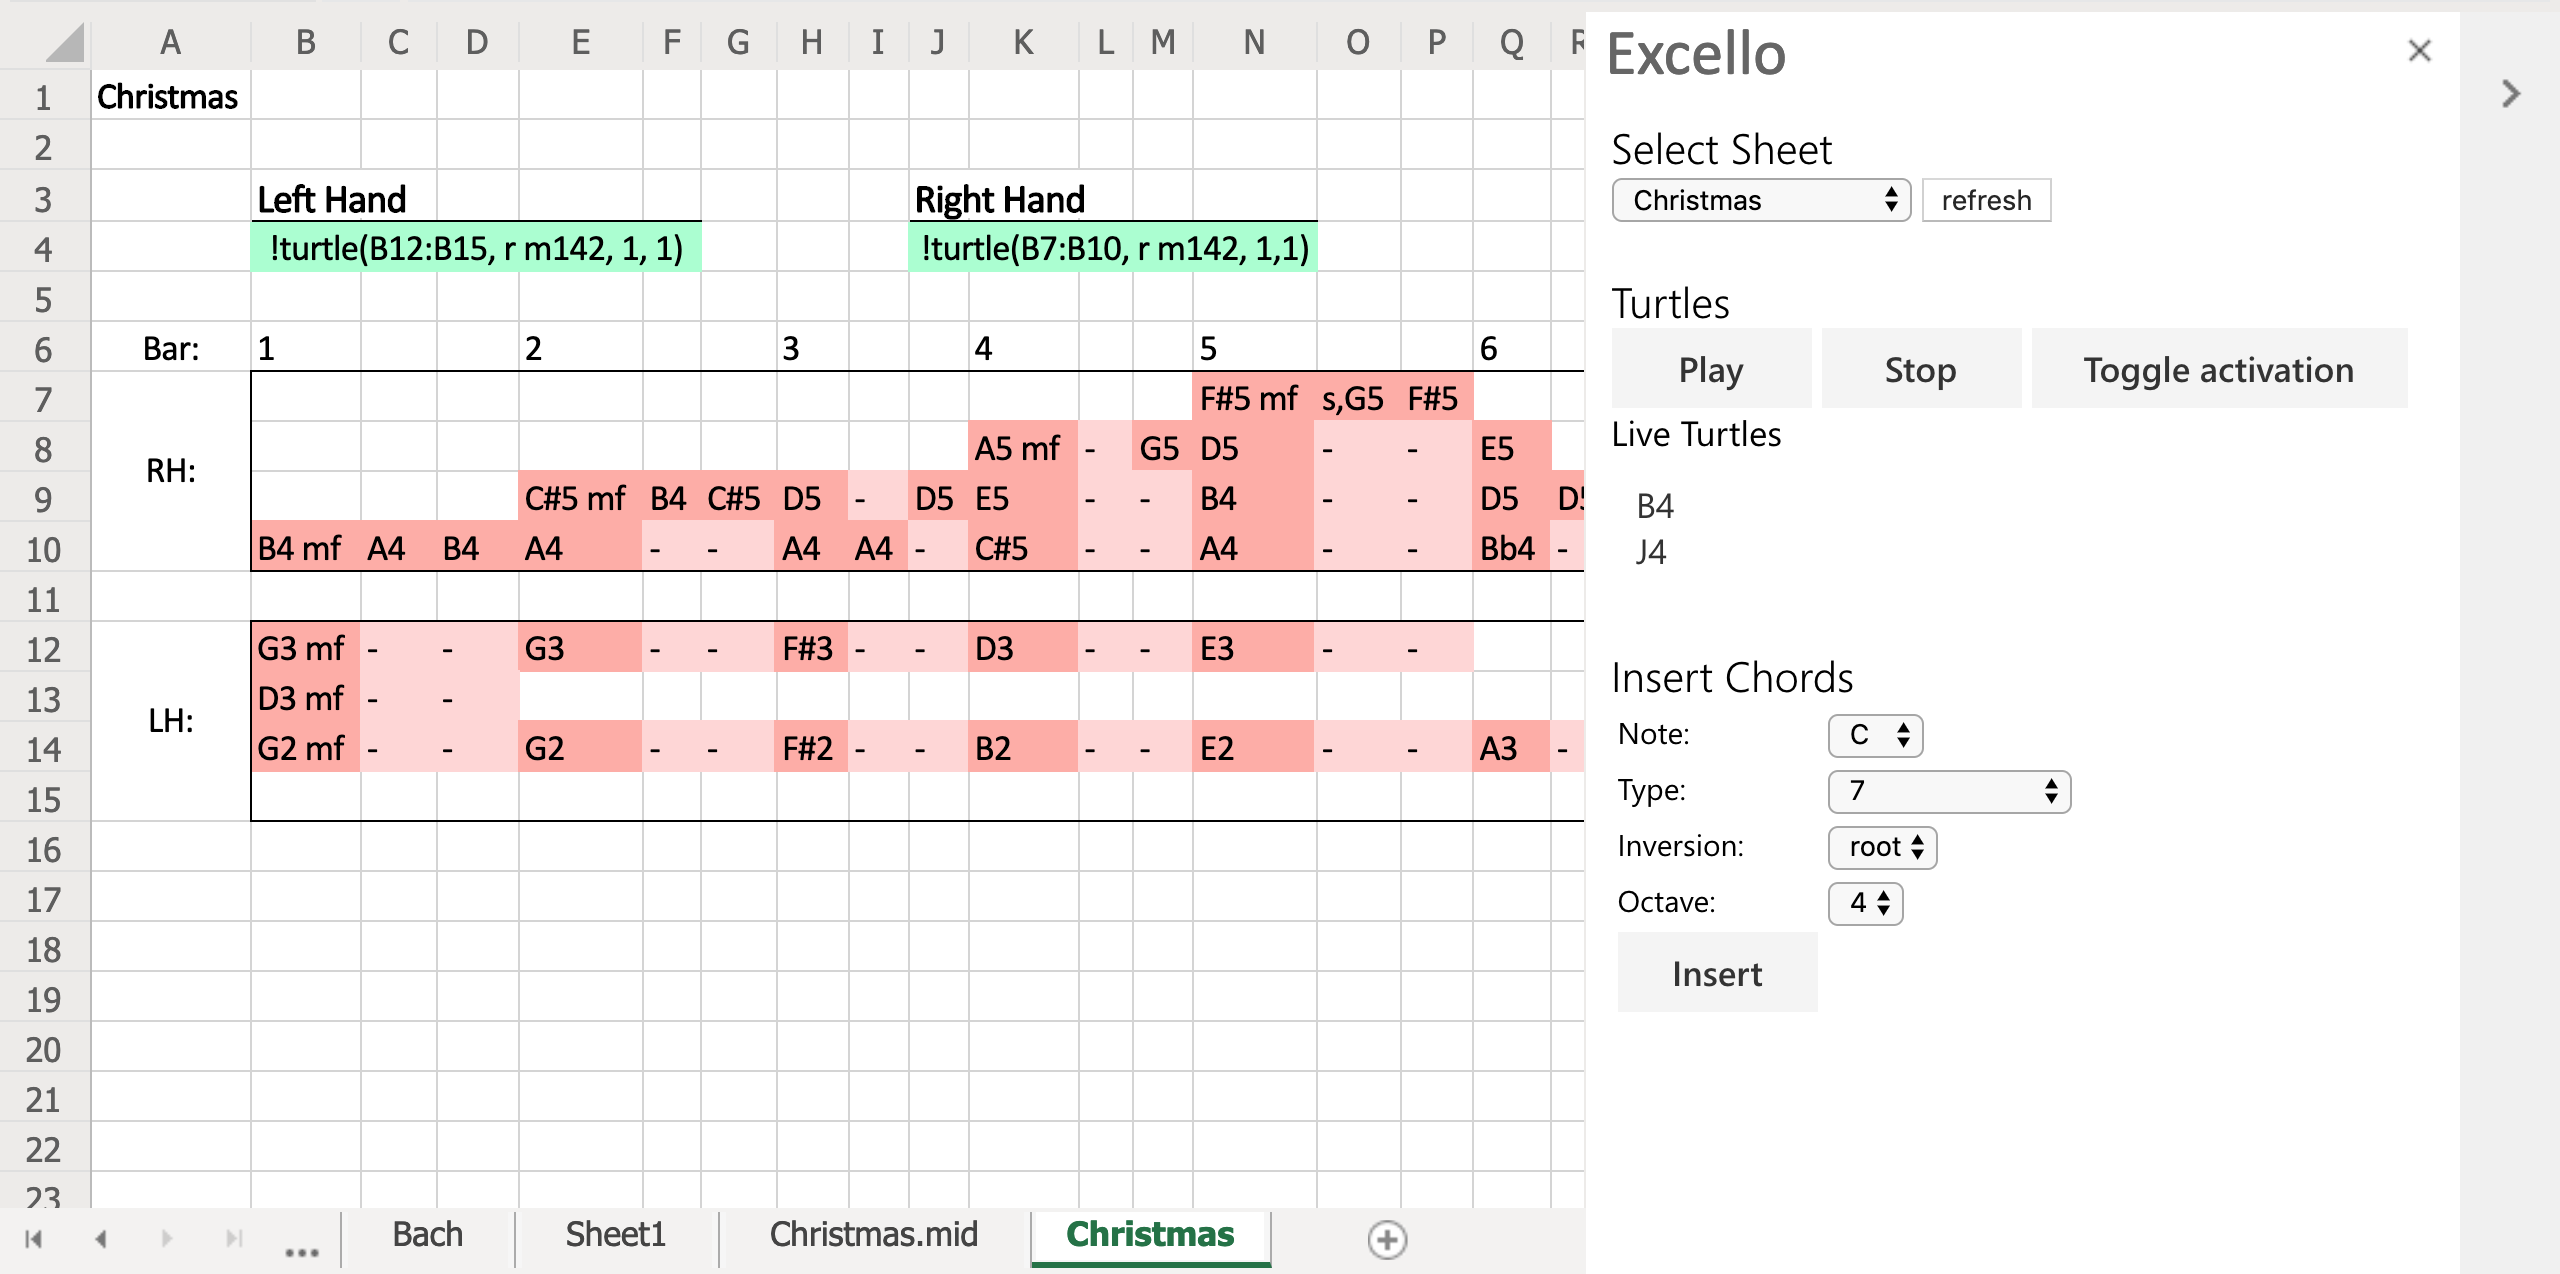
\includegraphics[width=150mm]{figs/excello.png}}
\caption{The Excello notation and add-in}
\label{intro:excello}
\end{figure}

\section{Outline of work}

\begin{enumerate}
\item I design a system for musical expression and playback within Excel. An initial prototype is built satisfying the all the success criteria of the system itself: play individual notes and chords with defined durations, define multiple parts, play loops, define sequences of notes and chords and be able to call these for playback, and define the tempo of playback.

\item Participatory design commences using the initial prototype as a discussion point. Following formative evaluation sessions with 21 participants, issues and feature requests are identified. Users continue to use the system and give feedback following their introductory session.

\item A series of additional extensions are implemented to solve the problems identified by participants and add features that are requested to improve the system.

\item A converter from MIDI to the Excello format is built to aid in the translation of a large existing corpus of MIDI files to the Excello notation.

\item Summative evaluation is carried out with the participants. The success of the features implemented as part of the participatory design phase is evaluated. The usability of Excello is analysed using the Cognitive Dimensions of Notation (CDN) framework \cite{blackwell:tutorial}, focusing on Sibelius as a comparison.

\end{enumerate}
